\documentclass[11pt]{article}

\usepackage{amsmath}
\usepackage{amssymb}
\usepackage{amsfonts}
\usepackage{amsthm}
\usepackage{backnaur}
\usepackage[scaled]{beramono}
\usepackage{bm}
\usepackage[small,bf]{caption}
\usepackage[strict]{changepage}
\usepackage{dblfloatfix}
\usepackage{enumerate}
\usepackage{enumitem}
\usepackage{flushend}
\usepackage[T1]{fontenc}
\usepackage{graphicx}
\usepackage{ifsym}
\usepackage{lipsum}
\usepackage{listings}
\usepackage{makeidx}
\usepackage{mathrsfs}
\usepackage{multirow}
\usepackage{pdfpages}
\usepackage{subcaption}
\usepackage{setspace}
\usepackage{textcomp}
\usepackage[hyphens]{url}
\usepackage{booktabs}
\usepackage{multirow}
\usepackage{xcolor}
\usepackage{pgfgantt}
\usepackage{wrapfig}
\usepackage{balance}
\usepackage{tikz}
\usetikzlibrary{shapes,decorations}
\usepackage{pgfplots}
\usepgfplotslibrary{units}
\pgfplotsset{compat=1.14}
\usepackage{bm}
\usepackage[
backend=biber,
style=ieee
]{biblatex}
\usepackage{hyperref}
\hypersetup{
    colorlinks=true,
    linkcolor=blue,
    filecolor=magenta,
    urlcolor=cyan,
}
\addbibresource{references.bib}

\newcommand{\rt}{\textsuperscript{\textregistered}}
\newcommand{\tm}{\texttrademark}

\addtolength{\evensidemargin}{-.5in}
\addtolength{\oddsidemargin}{-.5in}
\addtolength{\textwidth}{0.8in}
\addtolength{\textheight}{0.8in}
\addtolength{\topmargin}{-.4in}
%%%%%%%%%%%%%%%%%%%%%%%%%%%%%%
%%%%%%%%%%%%%%%%%%%%%%%%%%%%%%
%%%%%%%%%%%%%%%%%%%%%%%%%%%%%%
\title{\vspace{-25pt}
\huge CS 15-618 Project Report \\
\huge Synchrony (ID 24)
}
\author{
    Patricio Chilano (pchilano) \\
    Omar Serrano (oserrano)
}
\date{\today}

\begin{document}

\definecolor{beaublue}{rgb}{0.74, 0.83, 0.9}

\lstset{
    language=C++,
    basicstyle=\ttfamily\scriptsize,
    keywordstyle=\color{blue}\ttfamily,
    stringstyle=\color{red}\ttfamily,
    commentstyle=\color{orange}\ttfamily,
    morecomment=[l][\color{magenta}]{\#},
    breaklines=true,
    morekeywords={nullptr,noexcept}
}

\maketitle

\section*{Summary}

\section*{Background}

\section*{Approach}


Lockfree lists were implemented based on \cite{Harris}.  If a list would only
expose the Insert() and Find() methods it would be trivial to implement without
using locks. The only operation that we would need to worry about in a
concurrent environment is the Insert() one, for which we would only need to
update a pointer atomically. This can be done using a CAS instruction that would
retry the opertion in case the pointer to be updated happens to change in the
middle of the operation. The real challenge with removing locks from the
implementation of a list has to do with the Remove() operation. In order to
guarantee that no extra nodes are inserted concurrently after a node being
deleted, and thus corrupting the list, it would seem that we would need a DCAS
operation, i.e. an atomic compare and swap that would simultaneously update the
next pointer of the node being removed and the next pointer of its previous
node. With the algorithm proposed by Harris the Remove() operation can be
accomplished with only a single CAS, by means of dividing the delete operation
in a logical delete and a physical delete. The key idea is to use the unused
lower bits in the value of the pointer to the next node to store a flag that
would mark the node as deleted. Deleting the node would first make a logical
remove by marking its pointer to next node, and finally the actual physical
remove from the list would be done. Since the logical remove just changes unused
bits from the pointer of the deleted node other threads can still traverse the
list ignoring logical removed nodes, thus mantaining concurrency  and
correctness.

Describe the technologies used. What language/APIs? What machines did you
target?

Describe how you mapped the problem to your target parallel machine(s).
Important: How do the data structures and operations you described map to
machine concepts like cores and threads. (or warps, thread blocks, gangs, etc.)
Did you change the original serial algorithm to enable better mapping to a
parallel machine? If your project involved many iterations of evaluation and
optimization, please describe this process as well. What did you try that did
not work? How did you arrive at your solution? The notes you’ve been writing
throughout your project should be helpful here. Convince us you worked hard to
arrive at a good solution. If you started with an existing piece of code, please
mention it (and where it came from) here.

\section*{Results}

\section*{Conclusion}

\section*{Division of Work}
Equal work was performed by both partners.

%lateday_combined_list_insert_10_lookup_10_removal_80.png
%lateday_combined_list_insert_10_lookup_80_removal_10.png
%lateday_combined_list_insert_25_lookup_25_removal_50.png
%lateday_combined_list_insert_25_lookup_50_removal_25.png
%lateday_combined_list_insert_50_lookup_25_removal_25.png
%lateday_combined_list_insert_80_lookup_10_removal_10.png

%lateday_combined_map_insert_10_lookup_10_removal_80.png
%lateday_combined_map_insert_10_lookup_80_removal_10.png
%lateday_combined_map_insert_25_lookup_25_removal_50.png
%lateday_combined_map_insert_25_lookup_50_removal_25.png
%lateday_combined_map_insert_50_lookup_25_removal_25.png
%lateday_combined_map_insert_80_lookup_10_removal_10.png

\begin{figure}[h]
\centering
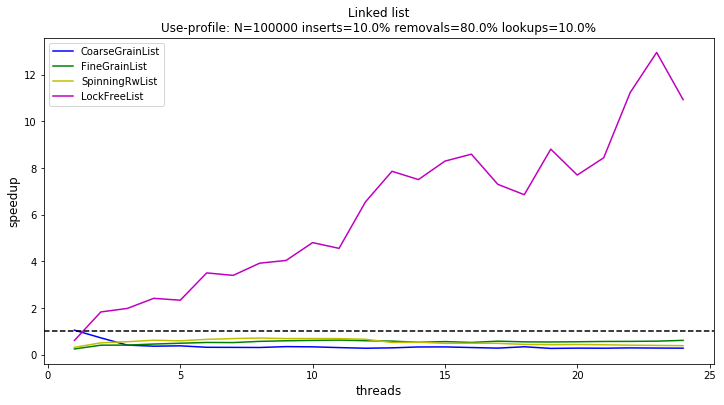
\includegraphics[width=1.0\linewidth]{figs/lateday/combined/lateday_combined_list_insert_10_lookup_10_removal_80}
\caption{Fig.}
\label{fig:fig1}
\end{figure}

\begin{figure}[h]
\centering
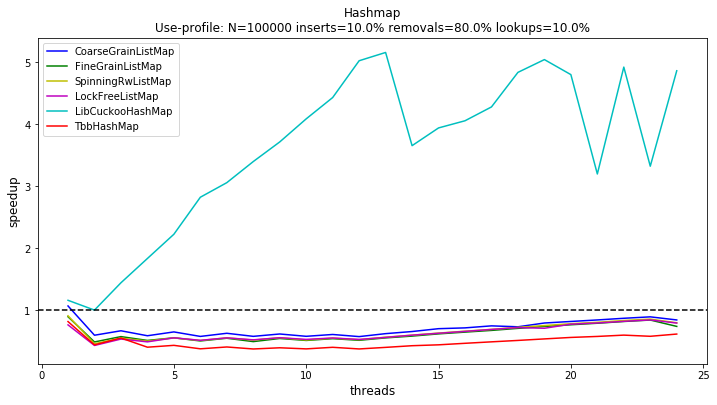
\includegraphics[width=0.5\linewidth]{figs/lateday/combined/lateday_combined_map_insert_10_lookup_10_removal_80}
\caption{Fig.}
\label{fig:fig2}
\end{figure}

\printbibliography

\end{document}
